\subsubsection{Programmets opbygning}

Programmet er opbygget efter desginprincippet "top-down programmering".Princippet går ud på at dele programmet op i mindre dele, og derefter løse de mindre dele i hver deres funktion. Funktionerne samles i main, som kun bruges til kommunikation med brugeren. Figur \ref{fig:topdown} viser tankegangen bag top-down programmering, hvor de enkelte problemer deles op og løses som delproblemer. 

\begin{figure}[H]
    \centering
    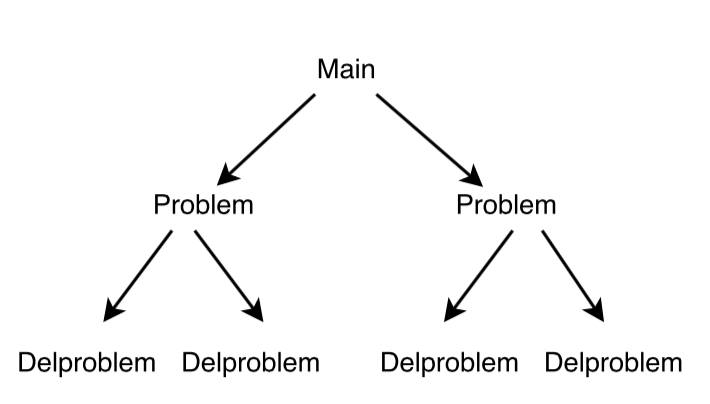
\includegraphics[width=10cm]{topdown}
    \caption{Tankegangen bag top-down programmering.}
    \label{fig:topdown}
\end{figure}

Som en del af vores top-down fremgangsmåde har vi struktureret opgaven i header-filer som blandt andet indeholder prototyper og structs. Header-filerne hjælper os med, at få bedre overblik over koden. 
